%% ============================================================================
%%
%%  Part A / PhD Progress Report
%%
%%  Author: Jakob Lysgaard Rørsted (Mosumgaard)
%%
%%  IMPORTANT: Compile with pdfLaTeX+biber !
%%
%%  Remarks:
%% - Needs to be executed with '--shell-escape' if the minted-package is used!
%%
%% ============================================================================

% ~~~~~~~~~~~~~~~~~~~~~~~~~~~~~~~~~~~~~~~~~~~~~~~~~~~~~~~~~~~~~~~~~~~~~~~~~~~~~
% Preamble and input control
% ~~~~~~~~~~~~~~~~~~~~~~~~~~~~~~~~~~~~~~~~~~~~~~~~~~~~~~~~~~~~~~~~~~~~~~~~~~~~~

% Use memoir!
\documentclass[%
final,
11pt,
% openright,
openany,
twoside,
british,
a4paper
]{memoir}

% Global definition: Name of the project (e.g. for the headers)
\newcommand{\projecttitle}{Towards trapping of molecular ions in a linear Paul Trap}

% Read the actual preamble
%% ============================================================================
%%
%%  Part A / PhD Progress Report
%%
%%  Author: Jakob Lysgaard Rørsted (Mosumgaard)
%%
%%  Preamble
%% ============================================================================

% ~~~~~~~~~~~~~~~~~~~~~~~~~~~~~~~~~~~~~~~~~~~~~~~~~~~~~~~~~~~~~~~~~~~~~~~~~~~~~
% Core
% ~~~~~~~~~~~~~~~~~~~~~~~~~~~~~~~~~~~~~~~~~~~~~~~~~~~~~~~~~~~~~~~~~~~~~~~~~~~~~
% Essentials
\usepackage[utf8]{inputenc}
\usepackage[T1]{fontenc}

% Microtype -- Subliminal refinements towards typographical perfection
\usepackage{microtype}
\microtypesetup{final}
% \microtypesetup{tracking = true}

% Various tools needed in the preamble and by some packages
\usepackage{etoolbox}

% Inclusion of code
% --> Needs to be loaded this early to avoid problems with some font packages
% NOTE: This packages requires the Python-module 'Pygments' to be installed
% NOTE: Fails unless this file is compiled with '--shell-escape' !
% \usepackage{minted}
% \usemintedstyle{friendly}

% Language (has to be loaded before the fonts..?)
\usepackage{babel}

% Fonts
\usepackage{libertine}            % Linux Libertine as text font
\usepackage{libertinust1math}     % Math support for Linux Libertine
\usepackage[scaled=.95]{newtxtt}  % Pretty teletype in correct size


% ~~~~~~~~~~~~~~~~~~~~~~~~~~~~~~~~~~~~~~~~~~~~~~~~~~~~~~~~~~~~~~~~~~~~~~~~~~~~~
% Page 'n' stuff
% ~~~~~~~~~~~~~~~~~~~~~~~~~~~~~~~~~~~~~~~~~~~~~~~~~~~~~~~~~~~~~~~~~~~~~~~~~~~~~
% Page set-up
\setlrmarginsandblock{3.2cm}{*}{1.5}
\setulmarginsandblock{*}{3.7cm}{1}

% Some memoir tricks
\setlength{\topskip}{1.6\topskip}
\checkandfixthelayout
\sloppybottom
\strictpagechecktrue

% To remove the blank page after the titlepage to save space
% --> Only for this progress report! Normally the blank page should be there!!
\usepackage{atbegshi}


% ~~~~~~~~~~~~~~~~~~~~~~~~~~~~~~~~~~~~~~~~~~~~~~~~~~~~~~~~~~~~~~~~~~~~~~~~~~~~~
% Page and chapter styles
% ~~~~~~~~~~~~~~~~~~~~~~~~~~~~~~~~~~~~~~~~~~~~~~~~~~~~~~~~~~~~~~~~~~~~~~~~~~~~~

% NOTE: Colors added everywhere, to make them easy to change!
\usepackage{xcolor}

% Fonts
\newcommand{\foliofont}{\color{black}\sffamily}
\newcommand{\headerfont}{\color{black}\sffamily}
\newcommand{\kommentar{}}{\color{red}{}}
% Make new pagestyle
\makepagestyle{jrmbsc}
\makeevenhead{jrmbsc}{\foliofont\thepage}    {} {\headerfont\leftmark}
\makeoddhead {jrmbsc}{\headerfont\projecttitle} {} {\foliofont\thepage}
\makeevenfoot{jrmbsc}{}{}{}
\makeoddfoot {jrmbsc}{}{}{}

% Black magic happens below!
\makeatletter
\makepsmarks {jrmbsc}{
  % Syntax: \createmark{<division type}{left|right|both marks}{shownumber|nonumber}{prefix}{postfix}
  \createmark{chapter}    {both}  {shownumber} {\@chapapp\ } {\ $\cdot$\ }
  \createmark{section}    {right} {shownumber} {}            { \ }
%  \createmark{subsection} {right} {nonumber}   {}            {}
  \createplainmark{toc}   {both}  {\contentsname}
  \createplainmark{lof}   {both}  {\listfigurename}
  \createplainmark{lot}   {both}  {\listtablename}
  \createplainmark{bib}   {both}  {\bibname}
  \createplainmark{index} {both}  {\indexname}
}
\makeatother
\nouppercaseheads

% Sections with sans-serif
\setsecheadstyle{\Large\bfseries\sffamily\raggedright}
\setsubsecheadstyle{\large\bfseries\sffamily\raggedright}
% \setsecheadstyle{\Large\sffamily\raggedright}
% \setsubsecheadstyle{\large\sffamily\raggedright}

% Fix of the chapter-pages
\copypagestyle{chapter}{empty}
\makeoddfoot{chapter}{}{\foliofont\thepage}{}
\makeevenfoot{chapter}{}{\foliofont\thepage}{}

% Chapterstyle (modified from Rasmus Villemoes thesis)
\usepackage{graphicx}
\makechapterstyle{jrmbsc}{% requires graphicx package
  \chapterstyle{default}
  \renewcommand*{\chapnamefont}{%
    \normalfont\LARGE\color{black}\scshape\raggedleft}
  \renewcommand*{\chaptitlefont}{%
    \normalfont\Huge\color{black}\sffamily\raggedleft}
  \renewcommand*{\chapternamenum}{}
  \renewcommand*{\printchapternum}{%
    \makebox[0pt][l]{\hspace{0.4em}
      \resizebox{!}{5ex}{%
        \normalfont\Large\color{black}\thechapter}
    }%
  }%
  \renewcommand*{\afterchapternum}{%
    \par\hspace{1.5cm}\color{black}\hrule\vskip\midchapskip}}

% Use the new pagestyle and chapterstyle
\pagestyle{jrmbsc}
\chapterstyle{jrmbsc}

% Turn on numbering of subsections
\setsecnumdepth{subsection}


% ~~~~~~~~~~~~~~~~~~~~~~~~~~~~~~~~~~~~~~~~~~~~~~~~~~~~~~~~~~~~~~~~~~~~~~~~~~~~~
% Floats, captions and footnotes
% ~~~~~~~~~~~~~~~~~~~~~~~~~~~~~~~~~~~~~~~~~~~~~~~~~~~~~~~~~~~~~~~~~~~~~~~~~~~~~
% Include graphics
% \usepackage{graphicx}  % ALREADY IMPORTED

% Subfloats
\newsubfloat{figure}
\subcaptionstyle{\raggedright}

% Use sans-serif for captions
\captionnamefont{\sffamily\scshape}
\captiontitlefont{\sffamily\small}

% Width of caption --> Use sf-font instead
% \captionwidth{.8\linewidth}
% \changecaptionwidth

% Trick to automatically end captions with a period
\captiontitlefinal{.}

% Styling of the footnotes (memoir tricks)
\setlength{\footmarkwidth}{-1sp}
\setlength{\footmarksep}{0em}
\footmarkstyle{#1: }

% Cool tables with footnotes (using the same style as define just above)
\usepackage[online]{threeparttable}
\appto\TPTnoteSettings{\footnotesize}


% ~~~~~~~~~~~~~~~~~~~~~~~~~~~~~~~~~~~~~~~~~~~~~~~~~~~~~~~~~~~~~~~~~~~~~~~~~~~~~
% Science
% ~~~~~~~~~~~~~~~~~~~~~~~~~~~~~~~~~~~~~~~~~~~~~~~~~~~~~~~~~~~~~~~~~~~~~~~~~~~~~
% Basic math
\usepackage{amsmath}

% Bad-ass math!
\usepackage{mathtools}
\mathtoolsset{showonlyrefs=false,showmanualtags}
% \mathtoolsset{showonlyrefs=true}  % If only to show numbers on ref'ed eq's

% Units
\usepackage{siunitx}
\sisetup{separate-uncertainty=true}

% Declaration of some nice units
\DeclareSIUnit\au{AU}
\DeclareSIUnit\year{yr}
\DeclareSIUnit\erg{erg}
\DeclareSIUnit\msun{M_{\odot}}
\DeclareSIUnit\lsun{L_{\odot}}

% Computer-related units
\DeclareSIUnit\byte{B}

% Delimeters
\DeclarePairedDelimiter\abs{\lvert}{\rvert}
\DeclarePairedDelimiter\norm{\langle}{\rangle}


% ~~~~~~~~~~~~~~~~~~~~~~~~~~~~~~~~~~~~~~~~~~~~~~~~~~~~~~~~~~~~~~~~~~~~~~~~~~~~~
% Stuff
% ~~~~~~~~~~~~~~~~~~~~~~~~~~~~~~~~~~~~~~~~~~~~~~~~~~~~~~~~~~~~~~~~~~~~~~~~~~~~~
% Spacing in macros
\usepackage{xspace}

% Debugging
\usepackage{lipsum}
\usepackage[margin,draft]{fixme}
\fxusetheme{color}
% \fxnote (grøn), \fxerror (gul), \fxwarning (orange), \fxfatal (rød)

% Things with draft
\usepackage[firstpage]{draftwatermark}
\SetWatermarkText{\sffamily DRAFT}

% Nice itemizations
\usepackage{enumitem}
% \firmlists  % Activate firmlists everywhere?

% Logo
\usepackage{metalogo}
\setlogokern{La}{-0.265em}
\setlogokern{aT}{-0.09em}
\setlogokern{Te}{-0.07em}
\setlogokern{eX}{-0.072em}
\setlogokern{eT}{-0.056em}
\setlogodrop{0.158em}

% ~~~~~~~~~~~~~~~~~~~~~~~~~~~~~~~~~~~~~~~~~~~~~~~~~~~~~~~~~~~~~~~~~~~~~~~~~~~~~
% References
% ~~~~~~~~~~~~~~~~~~~~~~~~~~~~~~~~~~~~~~~~~~~~~~~~~~~~~~~~~~~~~~~~~~~~~~~~~~~~~
% Smart quotations
\usepackage{csquotes}

% URL's
\usepackage{url}

% Bibliography
\usepackage[backend=biber,
  style=authoryear-comp,  % Citation style as (AUTHOR YEAR)
  sorting=ynt,     % Sort citations as YEAR-NAME-TITLE
  sortcites=true,
  dashed=false,
  maxcitenames=3,     % Increase/decrease to include more/fewer authors in cites
  maxbibnames=3,      % As above, but in the bibliography
  uniquelist=false,
  uniquename=false,
  doi=false,
  url=false,
  isbn=false,
  eprint=false,
  hyperref=true]{biblatex}

% Actually apply the citation order (because bibliography sorted differently)
\assignrefcontextentries[]{*}

% Manual entries
\addbibresource{bibliography.bib}

% The one from Mendeley
% \addbibresource{library.bib}

% Space in bibliography
\setlength\bibitemsep{1.1\itemsep}

% Change bib-order
\DeclareNameAlias{sortname}{last-first}

% Referencing packages (needs to be loaded in this order!)
% --> For references, use: \cref{}  or \Cref{} !
\usepackage{refcount}
\usepackage{varioref}
\usepackage[
  unicode=true,
  pdftitle={\projecttitle},
  pdfauthor={Emil Lenler-Eriksen},  % Change this name!
  pdfkeywords={},
  bookmarksopen=true,
  pdfdisplaydoctitle=true,
  hypertexnames=false,
  ]{hyperref}
\usepackage{cleveref}

% Hyperref setup (from Rasmus Villemoes)
\makeatletter
\@ifpackageloaded{hyperref}{
  \hypersetup{colorlinks=false, pdfborder=0 0 0}
  \addto\extrasenglish{ % What does this do???
    \renewcommand\subsectionautorefname{Subsection}%
    \renewcommand\sectionautorefname{Section}%
    \renewcommand\chapterautorefname{Chapter}%
    \renewcommand\equationautorefname{equation}%
  }
}{}
\makeatother


% ~~~~~~~~~~~~~~~~~~~~~~~~~~~~~~~~~~~~~~~~~~~~~~~~~~~~~~~~~~~~~~~~~~~~~~~~~~~~~
% Macros
% ~~~~~~~~~~~~~~~~~~~~~~~~~~~~~~~~~~~~~~~~~~~~~~~~~~~~~~~~~~~~~~~~~~~~~~~~~~~~~
% Nice spacing in macros
\usepackage{xspace}

% Small division
\newcommand\starbreak{\medskip\fancybreak{$*$\qquad$*$\qquad$*$}\medskip}

% Seperation in equation
\newcommand\eqsep{\ensuremath{\quad , \quad}}

% Generic names
\newcommand\numpy{NumPy\xspace}
\newcommand\scipy{SciPy\xspace}
\newcommand\kepler{\textsl{Kepler}\xspace}

% Diff
\newcommand\diff[2]{\frac{\text{d}#1}{\text{d}#2}}
\newcommand\pdiff[2]{\frac{\partial #1}{\partial #2}}
\newcommand\idiff[2]{\ensuremath{\text{d}#1/\text{d}#2}}

% More lazy stuff
\newcommand\parname[2]{\left(#1\right)_{\textup{#2}}}

% Vectors (we are doing physics!)
\renewcommand{\vec}[1]{\ensuremath{\boldsymbol{#1}}\xspace}

% Nice subscript
\newcommand\var[2]{\ensuremath{#1_{\textup{#2}}\,}\xspace}

% Specific abbreviations and names
\newcommand\eos{EoS\xspace}
\newcommand\gar{\textsc{garstec}\xspace}
\newcommand\Gar{\textsc{Garstec}\xspace}


% Specific things to be repeated often in the text
\newcommand\teff{\ensuremath{T_{\textup{eff}}}\xspace}
\newcommand\logg{\ensuremath{\log g}\xspace}

% Uncomment to include all  -->  Ugly hack, I know !
\renewcommand\includeonly[1]{}

% Which files to compile
\includeonly{%
  front/frontpages,
  main/intro,
  main/future,
}

% Make the fixme-package silent to avoid cluttering of the terminal output
% --> Comment-out to see the FiXme Summary as well as individual logs of
%     error/warning/fatal notes
% \fxsetup{silent}

% ~~~~~~~~~~~~~~~~~~~~~~~~~~~~~~~~~~~~~~~~~~~~~~~~~~~~~~~~~~~~~~~~~~~~~~~~~~~~~
% Contents
% ~~~~~~~~~~~~~~~~~~~~~~~~~~~~~~~~~~~~~~~~~~~~~~~~~~~~~~~~~~~~~~~~~~~~~~~~~~~~~

\begin{document}
% ~~~~~~~~~~~
% Frontmatter
% ~~~~~~~~~~~

% No frontmatter command to properly count pages for this specific report
% \frontmatter

% Frontpage and abstract
%% ============================================================================
%%
%%  Part A / PhD Progress Report
%%
%%  Author: Jakob Lysgaard Rørsted (Mosumgaard)
%%
%%  Front page, abstract and colophon
%% ============================================================================

% ~~~~~~~~~~~~~~~~~~~~~~~~~~~~~~~~~~~~~~~~~~~~~~~~~~~~~~~~~~~~~~~~~~~~~~~~~~~~~
% The title page
% ~~~~~~~~~~~~~~~~~~~~~~~~~~~~~~~~~~~~~~~~~~~~~~~~~~~~~~~~~~~~~~~~~~~~~~~~~~~~~

% Try to get rid of the blank verso
% --> Source: tex.stackexchange.com/questions/227711
\AtBeginShipoutNext{\AtBeginShipoutNext{\AtBeginShipoutDiscard}}

% The actual front page
\begin{titlingpage}
  \newlength{\frontpagecorrection}
  \calccentering{\frontpagecorrection}
  \begin{adjustwidth*}{\frontpagecorrection-2cm}{-\frontpagecorrection-2cm}

    \centering
    \sffamily

    \vspace*{0.1cm}

    \fontsize{26pt}{29pt}\selectfont

    \projecttitle \par

    \vspace{0.8cm}

    \fontsize{18pt}{22pt}\selectfont

    Emil Lenler-Eriksen \par

    \vspace{2.7cm}

    
\includegraphics[width=5cm]{front/segla1b}
%    \includegraphics[width=5cm]{figures/sac_trim}

    \vspace{2.7cm}

    PhD Progress Report

    \vspace{1.0cm}

    \fontsize{14pt}{17pt}\selectfont

    Department of Physics and Astronomy\par
    Aarhus University\par
    % Denmark

    \vspace{0.3cm}

    May 2024

  \end{adjustwidth*}
\end{titlingpage}


% ~~~~~~~~~~~~~~~~~~~~~~~~~~~~~~~~~~~~~~~~~~~~~~~~~~~~~~~~~~~~~~~~~~~~~~~~~~~~~
% The verso of the title page
% ~~~~~~~~~~~~~~~~~~~~~~~~~~~~~~~~~~~~~~~~~~~~~~~~~~~~~~~~~~~~~~~~~~~~~~~~~~~~~

% We actually want the page numbering to start at 1 at the front page in order
% to count pages for the GSST requirements !
\setcounter{page}{2}

% ~~~~~~~~
% Abstract
% ~~~~~~~~
\vspace*{0.5cm}
\section*{Abstract}
\thispagestyle{empty}

Spectroscopy of molecular ions has been carried out by physicists for centuries. However, there is a constant push towards performing these measurements at colder temperatures in order to allow for higher precision.
Most spectroscopic methods for molecules are limited to temperatures of a few Kelvin by buffer gas cooling.  However, if the molecules are trapped in a linear Paul trap, their motions can be cooled to the motional ground state by applying laser-cooling to a co-trapped atomic ion with suitable transitions.

The work presented in this report covers the basics of trapping ions in a linear Paul trap, briefly describing the trap we use here in Aarhus, as well as going over the dynamics of systems consisting of one or two ions.
In addition, there is a description of the molecular ion source, a so-called electrospray ionization (ESI) source, which we plan to use for providing the molecular ions for our experiments.
The working concept of ESI is briefly explained, while results from a characterization of one of the octopoles within the setup are shown and discussed. Notably we find that ions may be stored in the octopole for several hours, meaning that once the ESI instrument has been filled, it can be closed off and used as a sort of "secondary ion source" for experiments.

Furthermore, we discuss how to cool down a system consisting of an atomic and a molecular ion down to the motional ground state. Doppler cooling is used to cool the atomic ion down to the so-called Doppler temperature, which is 0.5 mK for Ba$^+$ ions. While the molecular ion is not directly affected by the Doppler cooling, Coulomb interaction with the cold atomic ion should transfer heat out of the molecule in a process called sympathetic cooling. When the ions approach the Doppler temperature, they start behaving like a harmonic oscillator, at which point sideband cooling can be performed to reach the motional quantum ground state.
While Doppler cooling and sideband cooling are suitable for the case of ions with similar charge-to-mass ratios, they become unfeasible (without modification) when the ratios change too much, as the motion of the ions will become uncoupled.
In order to solve this issue, we introduce theory for coupling any two motional modes of the ions by an external field, oscillating at the difference of their frequencies. This allows transfer of energy from hard-to-cool modes into easy-to-cool modes, allowing for quantum ground state cooling of all motional modes.

Finally, there is a brief section containing a conclusion on the report, and an outlook on how we aim to proceed in the next two years.

% ~~~~~~~~~~~~
% The colophon
% ~~~~~~~~~~~~

% Get font-info
\makeatletter
\edef\fontandleading{\@memptsize.0/\the\baselineskip}
\makeatother

% % Push to bottom of page and locally set indents
% \strut\vfill
% {
%   \setlength{\parindent}{0pt}
%   \addtolength{\parskip}{.6em}

%   \begin{center}
%     \bfseries\sffamily Colophon
%   \end{center}

%   \small

%   \textsl{\projecttitle}

%   \smallskip

%   PhD progress report by Emil Lenler-Eriksen.

%   The PhD project is supervised by Michael Drewsen

%   Typeset by the author using \LaTeX{} and the \textsf{memoir} document class,
%   using Linux Libertine and Linux Biolinum {\fontandleading}.

%   %Printed at Aarhus University
% }

% List of fixme-notes -- REMEMBER TO REMOVE!
%  --> When removed, things will end on the correct pages
% \listoffixmes

% Table of contents manually aligned with abstract
\clearpage
% \tableofcontents*
{\addtolength{\beforechapskip}{-2\baselineskip}\tableofcontents*}


% ~~~~~~~~~~~
% Mainmatter
% ~~~~~~~~~~~

% Since frontmatter is not set, no need to set mainmatter
% \mainmatter

% Introduction
%% ============================================================================
%%
%%  Part A / PhD Progress Report
%%
%%  Author: Jakob Lysgaard Rørsted (Mosumgaard)
%%
%%  Introduction
%% ============================================================================

\chapter{Introduction}
\label{chap:intro}
In the 1950s Wolfgang Paul invented the so-called Paul trap, for trapping charged particles within a quadrupolar electromagnetic field \cite{PaulTrap}. In 1989, he would go on
 to receive the Nobel Prize in physics, alongside Hans Dehmelt, "for the development of the ion trap technique" \cite{NobelPrize.org}.
 With the many technological and scientific advancements since the Paul trap's conception, among which the laser is an especially important one,
 it is now possible to trap, and cool single ions to their motional ground state \cite{WinelandSideband}.
 Such cold ions pose many interesting possibilities for science, as they make good candidates for atomic clocks \cite{King2022},
 or the basis for quantum computers \cite{ZiracZoller,Kielpinski2002}.

Paul traps are also used for the study of fluorescence of molecules in the gas phase \cite{Kjaer2021-lm},
where pulsed lasers can be used to excite large clouds of molecular ions, whose fluorescence spectrum may then be recorded and studied.
However, as most molecules lack the necessary energy level structure for laser cooling, the temperature of these experiments are limited by their cryogenic cooling environment.


The aim of my PhD thesis, is to expand our current setup, such that single molecular ions from an electrospray ionization source \cite{FennEsi} can be trapped in a linear Paul trap alongside a Ba$^+$ ion, and cooled to their motional ground state.
In such a setup we would like to investigate the molecules using a method called photon recoil spectroscopy \cite{PRS}.

This method functions by using the momentum kick associated with the molecule's absorption of light
as a measure of whether absorption has occurred. Readout is performed by addressing an electronic transition of a Ba$^+$ atom, which is trapped alongside the molecule, with a laser, that is red detuned by exactly one of the motional frequencies of the collective ion motion. Thus, excitation can only occur if the motion of the ions has been excited by an absorption event.


Directly applying this method to two-ion systems with large mismatches in mass-to-charge ratio is challenging, since the motions of the ions are only very weakly coupled, and thus the absorption kick will predominantly excite the motion of the molecule, which is not sensitive to the readout performed by a laser on the 
Ba$^+$ ion. Due to this issue I have been looking at, and developing, theory for how to transfer energy from one motional mode to another, to allow for efficient readout of the absorption kick.\medskip
\newline
\noindent\Large{\textbf{Outline of the report}}\newline
\normalsize The report is divided into 5 different chapters. \Cref{chap:intro} is a brief introduction to the field, some of the challenges I face, and what I hope to accomplish with my PhD.

\Cref{chap:LinTrap} describes the physics of trapping ions in a linear Paul trap and is split into two sections, the first describing the trapping of a single ion, while the latter derives the common motion of two ions in the trap.

Next is \cref{chap:ESI} which describes the electrospray ionization source, which is the source of molecular ions for the experiment. The first section of this chapter is an overview of the setup and the second contains a characterization of one of the octopole guides within the setup.

\Cref{chap:Cooling} describes the laser cooling necessary for reaching the motional ground state of a two-ion system. The first section contains the theory for Doppler cooling, which allows the ions to reach a temperature of $\sim$1mK. The second section describes sideband cooling, which is necessary for cooling the motion of the system to its quantum mechanical ground state. Finally, the 3rd section of the chapter talks on how one can couple the motion of the ions by using an external field, in order to improve the cooling of systems where the two ions have large differences their mass-to-charge ratios.

Finally, \cref{chap:future} gives a short plan of the work I plan to do in the latter half of my PhD studies here at Aarhus.




%Physics of the Paul Trap
\chapter{The Linear Paul Trap}
\label{chap:LinTrap}
\textcolor{red}{THIS SECTION CONTAINS INFORMATION ON THE PAUL TRAP}

\section{Single ion in a linear Paul Trap}

\section{Two ions in a linear Paul trap}





%Electrospray Chapter
\chapter{Electrospray ionization source}
\label{chap:ESI}

\section{Overview of the electrospray and its components}
As the source of molecular ions for the experiment we implement a so-called electrospray ionization (ESI) source \cite{FennEsi,Kjaer2021-lm}. At the time of writing, the ESI source is not connected to the rest of the setup, but an illustration of what the setup will look like when everything is connected can be seen on \cref{fig:fullSetup}.
\begin{figure}
    \centering
    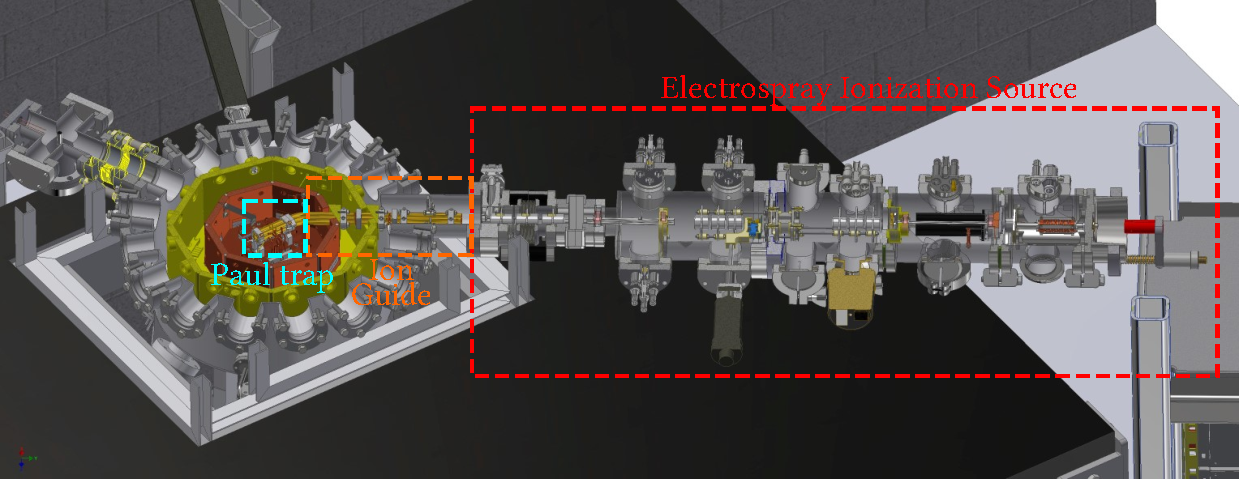
\includegraphics[width = 1.1\textwidth]{main/spray.pdf}
    \caption{3D figure of the full setup at Aarhus, when the electrospray (red) is connected to the cryogenic trap. The ion guide (orange) allows to transfer the ions into the cryogenic Paul trap (blue), where experiments will be conducted. At the time of writing the ESI source is not hooked up to the experiment, and instead there is channeltron detector at the very end of the electrospray, where it would connect to the ion guide}
    \label{fig:fullSetup}
\end{figure}


The basics of how such a device functions is that it has a syringe contains a solvent (typically methanol) with the ions one wishes to perform experiments on. The syringe is connected to a needle, and a motor slowly depresses the plunger on the spring, causing the solvent to form a droplet on the tip of the needle. The needle tip of the ESI source is sitting outside the vacuum chambers of the ESI setup, in atmospheric air.
Opposite of the needle is a narrow opening into the full body of the ESI source. The tip of the needle is put at a high voltage difference with respect to this opening (typically 3-3.5kV), this voltage difference leads to a strong electric field which will drag the charged droplets from the needle and into the opening of the instrument.
The ions then enter a capillary tube (see \cref{fig:esiDrawing}) heated to 70 degrees celsius, which is set at some voltage (typically 40V).
\begin{figure}
    \centering
    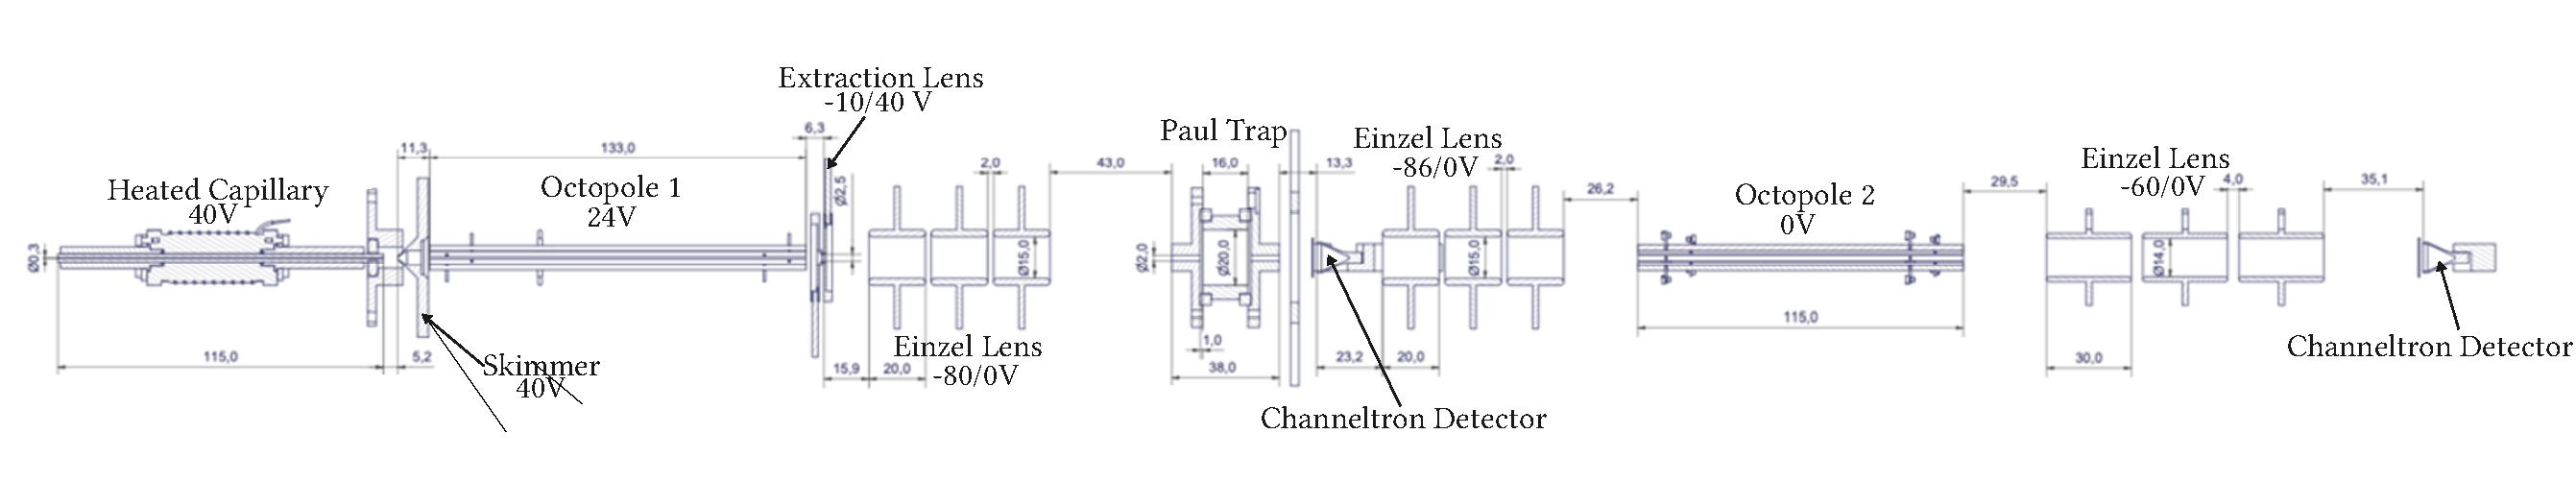
\includegraphics[width = 1.1\textwidth]{main/electrospray_elements.pdf}
    \caption{Technical drawing giving a sideview of all the components of the ESI source we employ. Some of the most important components on the figure have been labelled by name and the voltages typically emplyed on them.
    It is very important to ensure that there is a voltage gradient as one progresses down the ESI source, since otherwise the ions cannot travel. The multiple voltages noted for the Einzel lenses correspond to outer/inner electrode voltages, and for the extraction lens, the low voltage is set for extraction, while the high is for accumulation}
    \label{fig:esiDrawing}
\end{figure}
Within the heated capillary the solvent will begin to evaporate, causing the droplets to shrink. This causes the Coulomb repulsion of the ions within the droplet to increase as they all move nearer one another.
Eventually the surface tension of the droplet can no longer compensate the electrostatic repulsion of the ions within, and the droplet splits. This process repeats until all the solvent is evaporated and the ions are situated in the gas-phase. A schematic of this principle is illustrated on \cref{fig:evaporation}.
\begin{figure}
    \centering
    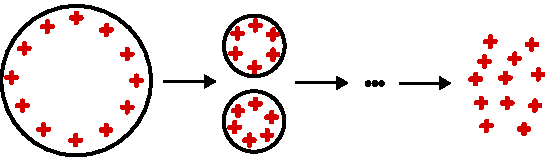
\includegraphics{main/evaporation.pdf}
    \caption{Illustration of the evaporation principle that allows for gas-phase ions in electrospraying. As the solvent evaporates, the droplet will shrink, until the surface tension becomes unable to counteract the electrostatic repulsion of the ions. This splits the droplet into two droplets, for which this process then repeats. Eventually all the solvent is evaporated and only gas-phase ions are left. Note that the number of ions within a droplet has been grossly underestimated for ease of illustration}
    \label{fig:evaporation}
\end{figure}

After the evaporation process, gas-phase ions travel past a skimmer and into an octopole storage device. The octopole allows for efficient transport of the ions across long regions, and acts as a source of buffer gas cooling down to room temperature, due to ion-neutral collisions with the atmospheric gas at a pressure of approx 1mbar. At the very end of the octopole is a pair of "extraction" electrodes (also called lenses). We have timed control of these electrodes, allowing us to accumulate ions in the octopole by setting a high voltage on them, and then releasing the ion bunch by lowering the voltage. We have performed several experiments on this part of the trap, to characterize the storage capabilities of the octopole, as well as the temporal shape of the ion bunches that arrive from it. The results of those investigations are found in \cref{sec:octopoleExperiments}.

Upon extraction from the octopole the ions pass through an Einzel lens. This is a set of three electrodes, where the outer two share the same voltage, and fulfills the same role for ions as a lens does for optics. We use the Einzel lens to focus down the ion beam onto the 2mm wide opening of a cylindrical Paul trap.

The cylindrical Paul trap has two different settings. The first is using it as an Einzel lens, where the front and back electrodes act as the outer electrodes, while the main cylinder acts as the center electrode. This setting uses no RF on the trap and just allows for a DC ion beam going through.
The other option is to utilize the RF on the Paul trap, in order to trap and store ions. Since we only need a single molecule within the cryogenic trap, we would like to be able to load ions into the Paul trap, and use it as a "secondary" ion source, extracting just a few ions at a time for experiments.
Additionally it is possible to leak in gas for buffer gas cooling of molecules stored in the cylindrical Paul trap.

Immediately after the Paul trap there is a channel electron multiplier detector (also referred to as a channeltron), which can measure the ion current. This detector has a push/pull feedthrough, allowing it to be moved in and out of the ion beam. This allows us to perform diagnostics on the components of the first half of the detector. Of course, if the detector is moved into the ion beam, there will be no ions further down in the setup.

If the first channeltron detector is not in the measurement position, the ions will continue down to another set of Einzel lenses, which focus them into a second octopole that moves them down to a final set of Einzel lenses, focusing them onto a 2nd channeltron detector. This 2nd detector allows us to measure the ion current that makes it all the way through the ESI part of the experiment.
It has to be noted, that the 2nd detector sits where the connection to the ion guide will eventually be mounted, and as such this is not a permanent installation, but only exists for testing parameters to ensure we are able to get ions to the very end of the ESI source.
\section{Experiments on the first octopole}
\label{sec:octopoleExperiments}
The need for getting only single molecular ions in our cryogenic Paul trap poses some very unique challenges for our ESI setup. Since these ion sources are built to maximize the number of ions moving through, we will need to have a very good understanding of the different parts of the electrospray in order to be able to tailor a protocol for getting single ions to our linear quadropole trap.
For this reason we have spent some time making a characterization of the very first octopole in the experiment. 
This section contains the results of these measurements. All measurements are performed on rhodamine 6G, since it sprays particularly well.

\subsection{Measuring the temporal shape of an ion bunch}
One of the first characterizations we perform is measuring the temporal shape of an ion bunch leaving the octopole.

To get such a measurement we allow ions to accumulate in the octopole for some set amount of time by setting the voltage on the extraction lens to 40V, until the ions are released by lowering the voltage to -10V. After some delay $\tau$ with respect to the release of the ions, the number of ions hitting the detector over a time interval of 50$\mu$s is then recorded. By repeating this method for several values of $\tau$ we are able to get a temporal shape of the ion bunch coming out of the octopole.
An illustration of the measurement sequence can be seen on \cref{fig:sequenceShape}. 

Since it is unclear how narrow the ion bunch is in time, the ion signal is adjusted such that when the electrospray is in the DC configuration a current of a few 100 ions per second is measured, this ensures the detector will not saturate.
\begin{figure}
    \centering
    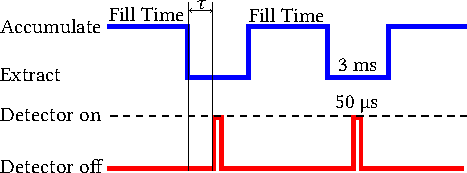
\includegraphics[width = 0.8\textwidth]{main/ShapePulse.pdf}
    \caption{Illustration of the experimental sequence for measuring the temporal shape of ion bunches leaving the first octopole (figure not to scale). Ions are accumulated (blue) over a preset time (data for 500ms, 30sec, and 1 minute were recorded) and then released. The measurement (red) is turned on for 50$\mu$s with a delay $\tau$ with respect to the release of the ions.
    Measurements are repeated 20 times for each value of $\tau$ in order to ensure good statistics. By varying $\tau$ and recording the number of ions a temporal shape of the ion bunch is recorded}
    \label{fig:sequenceShape}
\end{figure}

Results from the measurements when the octopole is allowed to accumulate ions for 500ms, 30 seconds and 1 minute can be seen on 
\cref{fig:bunchShape}. Here three loading times are compared, namely 500ms (green), 30 seconds (blue), and 1 minute (orange).
It is seen that the curves for 30 seconds and 1 minute are highly similar, this is likely because they contain very similar amounts of ions as can be seen on \cref{fig:fillTimeGraph}.

The 500ms curve is considerably slower than the other two, both in its rise time and its tail, by approximately a factor of 2. This indicates that the number of ions seems to affect the temperature, with fewer ions leading to colder temperatures.
Indeed, if we naively take the factor 2 difference in time constant to mean that the ions are half as slow, we find that if the ions are loaded for 500ms, they are about a quarter 
of the temperature of the ions that are loaded over 1 minute or 30 seconds.
\begin{figure}[h]
    \centering
    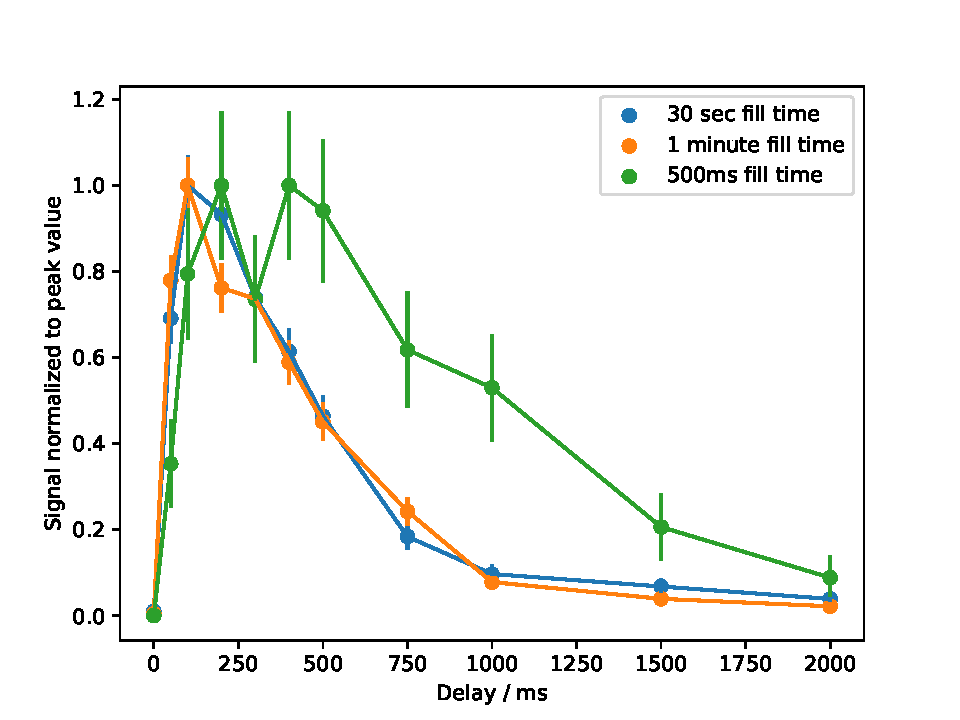
\includegraphics[width = 0.9\textwidth]{main/chargeShape.pdf}
    \caption{Plot showing the temporal shape of ion bunches, when the octopole is allowed to fill for 500ms (green), 30 seconds (blue), and 1 minute (orange).
    Each curve has been normalized to its peak value, in order to allow comparison of the curves. From the measurements it is clear that the majority of ions will arrive during the first milisecond if there are few ions in the octopole (500ms).
    The width of the pulse is shortened considerably down to approx 500ms if the octopole is allowed to fill. Thus if one wants to be careful of saturating the channeltron detector it is likely best to assume that when an ion bunch is released, all the ions will arrive during 500ms, as this allows some overhead.
    A feature to note is that the 500ms curve, seems to have a slope that is approx half as steep as the other two curves at the earliest part of the bunch.
    If one considers the tail we also see that the 500ms curve is approximately a factor two slower here as well. This gives a qualitative indication that loading fewer ions into the octopole, results in colder ions}
    \label{fig:bunchShape}
\end{figure}

It is not surprising to see that a higher number of ions in the octopole lead to higher temperatures. Firstly, the octopole is an RF device, and thus there will always be micromotion,
 (much like the quadrupole of \cref{chap:LinTrap}) for any ions that do not lie exactly on the center axis of the octopole. 
As more and more ions are loaded into the octopole, more of them will find their equilibria further off-axis, where the micromotion is larger, leading to hotter ions.

In addition, as the number of ions in the storage device increases, ion-ion collisions become more likely. It is known that such collisions in RF devices will lead to heating of the ion cloud \cite{BlumelHeating,MichaelIonIonHeating}.


\subsection{Measuring the fill time of the octopole}
Another characterization that has been performed, is testing how long it takes the octopole to reach the limit of the number of ions it can hold.
In order to test this, the octopole is allowed to fill for a variable time, after which the ions are released, and the channeltron detector records the total number of ions.
By doing this for increasing times, we expect to see a behaviour where the number of ions increases linearly in time initially, until space charge effects  eventually play a role.
When these effects become relevant, the loading of ions will become slower as new ions arriving knock "old" ions out of the octopole, until a steady state is realized.
An illustration of the experimental sequence can be seen on \cref{fig:storageSequence}. 

\begin{figure}
    \centering
    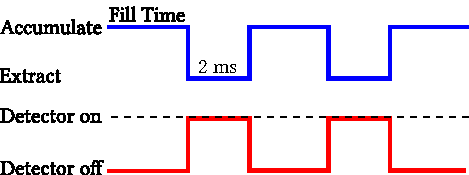
\includegraphics[width = 0.9\textwidth]{main/StoragePulse.pdf}
    \caption{Illustration (not to scale) of the measurement sequence used to obtain the results of this subsection. The octopole is allowed to fill with ions for variable times. The octopole is allowed to open for 2 ms, which is sufficient to let all the ions leave (see \cref{fig:bunchShape}). During the time when the octopole is open,
    the channeltron detector is turned on, to count the number of ions. For each fill time this procedure is repeated 20 times}
    \label{fig:storageSequence}
\end{figure}
All measurements for this experiment were taken at an ion current of approx 300 ions/second, measured at the channeltron detector.
The ion current measured at the detector usually varies within 10\% due to fluctuations in flow from the electrospray. Thus, any measurements of how long it takes to fill the octopole have to be adjusted for the ion flux during the loading phase.  This adjustment is done by multiplying the physical loading time by the ratio between the reference of 300 ions/s and the mean of the measured current before and after the measurement giving
\begin{equation}
    \tau'= \frac{I_{reference}}{I_{measured}}\tau,\quad I_{measured} = \frac{I_{before}+I_{after}}{2}.
\end{equation}
Results from the experiment with the time-axis adjsuted as described above can be seen on \cref{fig:fillTimeGraph}. From this, a very rough estimate of the ion current entering the octopole.
The density of ions in an octopole, where space-charge effects are included, can be written \cite{MajimaDensity}
\begin{equation}
    n(r) = \frac{144\epsilon_0 V_{RF}^2}{m\Omega^2r_0^4}\bigg(\frac{r}{r_0}\bigg)^4,
\end{equation}
where $V_{rf}$ is the RF voltage of the octopole (170V), $m$ is the mass of the ion (479 amu), $\Omega$ is the frequency of the octopole RF voltage ($2\pi\times2.7$MHz) and $r_0$ is half the distance between opposing octopole rods (2.75mm).


To obtain the linear density this has to be integrated this in the radial plane.
Of course the ions within the trap are unlikely to go all the way out to the electrodes, so there is the question of how far one sohuld integrate. Gerlich suggests that the ions can be stored out to $r = 0.8r_0$, by geometric considerations \cite{Gerlich1992}. We use this as it is an easy bound to implement. However the cutoff radius of the ion cloud might become more complex to describe when we are in the 
space-charge dominated regime \textcolor{red}{CITE MAJIMA}, as is the case when the octopole is full. We find the number of ions held in the octopole (length of 133mm) to be
\begin{equation}
    N = \frac{48\pi\epsilon_0V_{RF}^2L}{m\Omega^2r_0^2}\bigg(\frac{4}{5}\bigg)^6\approx 7.77\times 10^8.
\end{equation}
Again this number is likely to be lower in reality, but gives a ballpark figure for the number of ions that can be stored in the trap. Assuming the trap is full after 45 seconds of accumulation, we find there is a current of approx. $17\times 10^6$ ions/s entering the octopole while the electrospray is turned on.


\begin{figure}
    \centering
    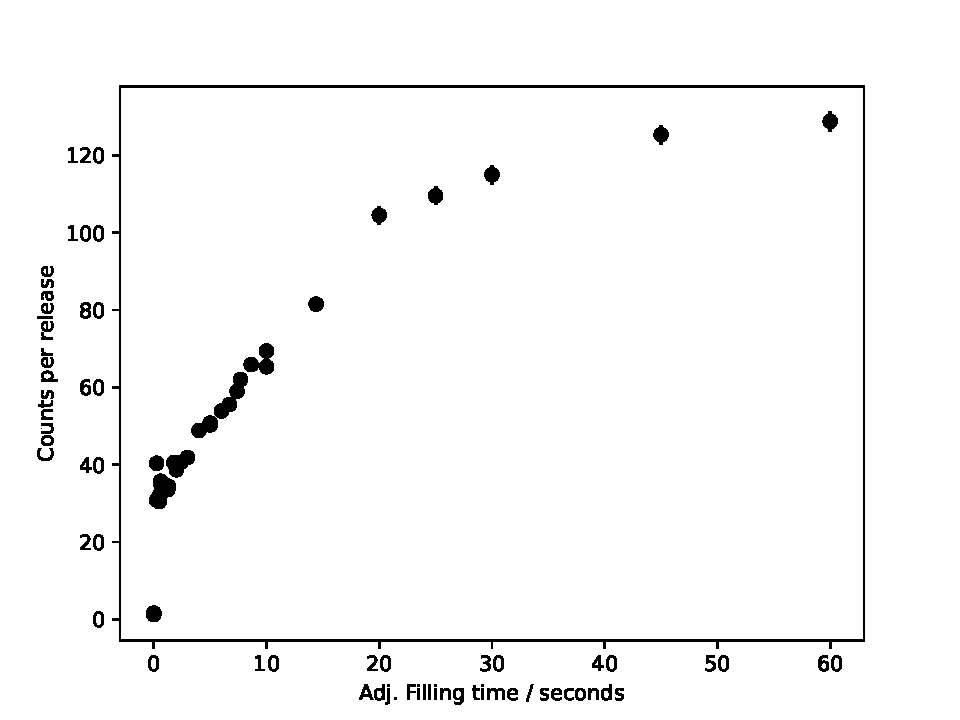
\includegraphics[width = 0.8\textwidth]{main/FillingTimeGraph.pdf}
    \caption{Results of the measurement of filling time of the octopole. For very low fill times there seems to be a very rapid increase in signal, which then becomes linear until approx. 15 seconds. After this the curve starts tapering off as the number of ions in the detector starts capping out in the mid-late 40s range}
    \label{fig:fillTimeGraph}
\end{figure}
\subsection{Storage time of the octopole}
The final measurement that has been performed on the first octopole aims to determine the period of time, in which ions can be kept in the octopole. Since the the electrospray setup is open to atmosphere, the pumps in the setup have to work hard to ensure low pressure at the end of the setup.
If the ions can be stored in the octopole for sufficiently long periods of time, that experiments may be performed using only the ions stored in the octopole, then it is possible to plug the opening of the electrospray, allowing for better vaccuum in the system.

In order to measure the lifetime of ions stored in the octopole, we allow the ions to accumulate in the octopole for 25 seconds after which we turn off the ion current into the octopole, by increasing the voltage on the skimmer to 200V.
An illustration of the experimental sequence can be found on \cref{fig:decaySequence}.
\begin{figure}[h]
    \centering
    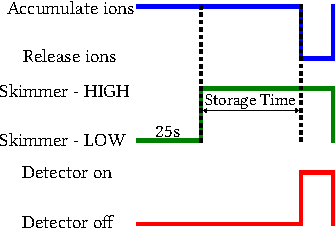
\includegraphics[width = 0.7\textwidth]{main/decayPulse.pdf}
    \caption{Illustration of the experimental sequence for measuring lieftime of ions in the octopole. The octopole (blue) is set to its accumulation voltage initially. The skimmer (green) is set to a low voltage of 40V for 25 seconds, allowing ions to enter the octopole. After 25 seconds have passed a voltage of 200V is applied to the skimmer. This blocks ions from entering the octopole.
    The ions are then kept in the octopole for a time, which is varied for each measurement, after which the ions are released and measured at the detector (red). Measurement is only performed once for the majority of timestamps.}    
    \label{fig:decaySequence}
\end{figure}
\begin{figure}[h]
    \centering
    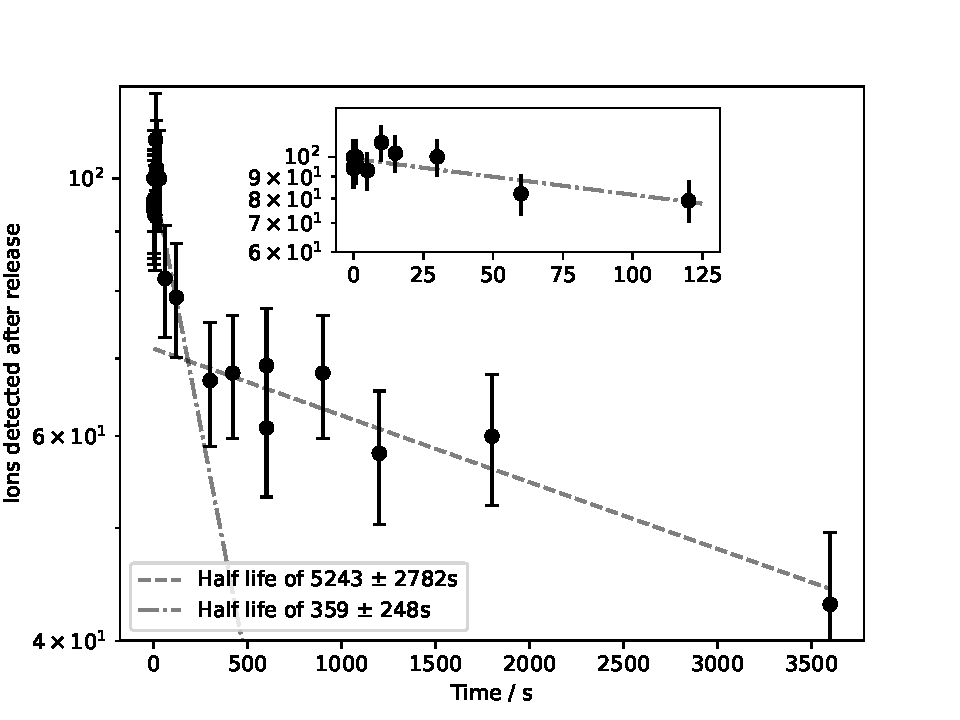
\includegraphics[width = 0.8\textwidth]{main/DecayTimes.pdf}
    \caption{Measurements of the lifetime of ions in the octopole. There clearly appear to be two timescales. At the short timescale (see inset), the number of ions in the octopole appear to be decaying with a half-life on the order of magnitude of minutes (dashed-dotted line). Conversely for longer timescales the rapid decay is no longer present and instead the population in the trap is decaying on the scale of hours (dahsed line).
    The cause for the initial rapid loss of population is likely ion-ion collisions within the trap, as the internal dynamics in the trap are initially dominated by space-charge effects. Eventually the ion density becomes sufficiently low to the point where the ions no longer feel one another, and instead losses are dominated by collisions with the background gas.}
    \label{fig:decayResults}
\end{figure}
Experimental results are seen on \cref{fig:decayResults}. From the figure it is evident, that there are two timescales at play, when determining the lifetimes of the ions.
For the first two minutes there is a rapid loss of ions, which if fitted to an exponential curve leads to a half of $359\pm249$s. After the heavy losses in the first few minutes the curve flattens out considerably. If an exponential decay is fitted to this part of the data a half life of $5243\pm2782$s is obtained. The reason for the large uncertainties in the half lives is that the statistics for the data aren't very good. Especially for the measurements at high storage times, data acquisition times become prohibitve
as a single measurement takes an upwards of an hour.

The fact that there are two timescales at play indicates that space-charge effects are important when the octopole is full. A possible explanation for why the ions die off as they do, is that initially the ions are experiencing ion-ion collisions, causing heavy losses on the time-scale of minutes.
As more and more ions are lost, the density within the octopole drops to a point, where ion-ion interactions no longer dominate losses in the octopole.
At this point the losses will be largely due to ion collisions with the neutral background gas. The measurements indicate that the timescale of this process is on the scale of hours.
Thus, it will likely be possible to use the octopole as an ion storage device, allowing for the closing of the electrosapray after an initial loading.
Closing off the electrospray to atmosphere is even likely to improve the storage time in the octopole since the long-term storage is determined by collisions with atmospheric air. The lower pressure obtained when the electrospray should lower the rate of collisions, and thus further minimize losses.

%Cooling physics
\chapter{Cooling}
\label{chap:Cooling}
A prerequisite for performing photon recoil spectroscopy, is that the system which is investigated, is cooled to the quantum mechanical ground state of its motion.
Cooling of ions in linear Paul traps usually occurs in two stages. First the ion(s) is cooled to approx. 1mK by Doppler cooling, as is described in \cref{sec:Doppler}.

When the ion(s) has been cooled to mK tempearture by Doppler cooling, it starts exhibiting quantum mechanical properties. Since the potential in the trap is harmonic, the wavefunction of the ion(s), is that of the harmonic oscillator.
To reach the quantum ground state, it is necessary to perorm sideband cooling which takes the ion(s) from whichever $\vert n\rangle$ state it starts in, and moves it to the state $\vert0\rangle$ of the harmonic oscillator. This process is described in \cref{sec:SBC}.

Finally there may be some complications to the above cooling processes if we consider two ions with very large charge-to-mass mismatch as explained in \cref{sec:2Ion}. \Cref{sec:Coupling}
\section{Doppler cooling}
\label{sec:Doppler}
The very first part of cooling two ions down consists of Doppler cooling \textcolor{red}{WINELAND}. This method of laser cooling was pioneered by David Wineland and relies on detuning laserlight with respect to an internal transition of the ion, in order to effectively generate a drag force on the ion, cooling it down.

An ion in motion experiences, with a velocity $\vec{v}$, experiences a Doppler shift of laser light with wave vector $\vec{k}$ according to
\begin{equation}
    \omega_{obs} \approx (1-\vec{k}\cdot\vec{v})\omega_L,
\end{equation}
where $\omega_{obs}$ is the frequency seen by the ion, and $\omega_L$ is the frequency of the laser in the laboratory frame.
Thus if we detune the light of the laser to be below the frequency of an electronic transition in the ion $\omega$, the ion will preferentially absorb photons, when it is propagating against the direction of the light.
Due to conservation of momentum, the ion must change its momentum by
\begin{equation}
    \Delta\vec{p} = \hbar\vec{k}.
\end{equation}
After a short time the ion will decay to the ground state once again, but since the direction of the photon emitted during decay is symmetric, this will, if averaged over multiple emissions, lead to no change in momentum.
Thus the momentum of the ion is effectively decreased, since the ion preferentially absorbs photons propagating in the oppsite direction of itself. At low velocities $kv\ll\Gamma$, where $\Gamma$ is the decay rate of the excited state, one can express this as a drag force (assuming 1D problem to ease notation) \textcolor{red}{KARIN}:
\begin{equation}
    F_{drag} = -\beta v,\quad \beta = \frac{8\hbar s k^2\delta / 2\Gamma}{\big(1+s+(2\delta/\Gamma)^2\big)^2},
\end{equation}
where $\beta$ is the drag coefficient, $\delta = \omega_L-\omega$ is the detuning of the laser with respect to the atomic transition, $s = I/I_{sat}$ is the saturation parameter, where $I$ is the intensity of the laser light, and $I_{sat} = \frac{\pi hc}{3\lambda}\Gamma$, with $\lambda$ being the wavelength of the laser, is the saturation intensity of the transition. 

It is important to note, that while the equation above seems to indicate that there is no limit to Doppler cooling, that is far from the case. Indeed since the direction of an emitted photon is random, the ion will perform a random walk in momentum space over time.
Thus, there is an intrinsic variation of velocity over time, meaning there is a lower limit to the temperature of the ion (typically referred to as the Doppler temperature or Doppler limit), which is given by
\begin{equation}
    T_D = \frac{\hbar\Gamma}{2k_b}\label{eq:DopplerTemp},
\end{equation}
which for the case of Ba$^+$ this temperature is approx. 0.5mK.

Of course Doppler cooling only works for very specific ions, that have the proper level-scheme, and is thus not a very good candidate for cooling arbitrary molecular ions.
The solution to this problem of not being able to doppler cool molecular ions comes in two parts. Firstly at high temperatures the hot molecular ion will interact with the cooled atomic ions, via the Coulomb interaction. Such interactions will cause the molecular ion to transfer energy to the atomic ion, from which the energy will then be removed by the system via Doppler cooling. This method of cooling is called sympathetic cooling \textcolor{red}{CITE MICHAEL (2000) AND REVIEW by Willitsch}
In this case we imagine ideally trapping the molecule with a large amount of Ba$^+$ ions to offer the most cooling.

As temperatures drop low enough that the motion truly becomes harmonic, the motion of the ions becomes coupled. As such, the ions will have common motional modes, and any energy extracted from the Ba$^+$ ion is extracted from the mode as a whole, thus cooling the molecular ion as well.
This cooling mechanism is only effective if the ions share similar mass-to-charge ratios, however. In the case where the ion motions are nigh uncoupled, as described in \cref{sec:2Ion}, further steps must be taken to get the molecular ion to mK temperatures. This is described in \cref{sec:Coupling}.


\section{Sideband Cooling}
\label{sec:SBC}
Unfortunately, Doppler cooling is not sufficient for reaching the motional ground state. In order to do this we employ yet another method of laser cooling, called sideband cooling \textcolor{red}{cite}. When the ions are at the doppler temperature, they will be cold enough that they behave as a quantum mechanical harmonic oscillator, with their wave function
being a thermal distribution over the Fock states $\vert n \rangle$. By coupling the state $\vert g,n\rangle$ to the state $\vert e,n-1\rangle$ where $(e,g)$ denotes the excited and ground states of the atom, we are able to remove one quanta of energy from the motion under an excitation of the electronic state.
Since the electronic state predominantly decays to the same $n$, this allows us to cool the ion's motion by moving down the "ladder" seen on \cref{fig:SBC}


We initially consider a single atomic ion in the Paul trap, and neglect the radial modes of motion in order to ease notation. The Hamiltonian can be written as
\begin{equation}
    \hat{H}_0 = \hbar\omega_{z}(\hat{n}+1/2)+\hat{H}_a,
\end{equation}
where $\hat{n}$ is the Fock state number operator, and $\hat{H}_a$ is the Hamiltonian for the atomic system. If a laser field is turned on at some detuning $\delta = \omega_L -\omega$ with respect to the electronic transition of the ion, the interaction with the laser in the interaction picture is described by:
\begin{equation}
    H_{I} = \frac{\hbar\Omega_0}{2}\hat{\sigma}_+\big(e^{ik_z\hat{z_I}}e^{-i\delta t}\big) + h.c.,
    \label{eq:interaction}
\end{equation}
where $\hat{\sigma}_+ = \vert e \rangle \langle g \vert$ is the excitation operator responsible for exciting the electronic state of the ion, and $\Omega_0 = \frac{eE_0}{\hbar}\langle g \vert \hat{\epsilon}\cdot\hat{z}\vert e\rangle$ is the Rabi frequency of the transition, being driven by an electric field of amplitude $E_0$, and direction $\hat{\epsilon}$. Note that the rotating wave approximation has been applied to the expression above, keeping only slowly rotating terms.

We may express $\hat{z}_I$ in terms of the ladder operators yielding
\begin{equation}
    \hat{z}_I = \sqrt{\frac{\hbar}{2m\omega_z}}(\hat{a}e^{-i\omega_z t}+\hat{a}^\dagger e^{i\omega_z t})
\end{equation}
Before inserting this expression back into \cref{eq:interaction}, it will be useful to first define the Lamb-Dicke parameter
\begin{equation}
    \eta = k_z\sqrt{\frac{\hbar}{2m\omega_z}},
\end{equation}
which in the so-called Lamb-Dicke regime, where $\eta\sqrt{\langle n \rangle +1} \ll 1$ \textcolor{red}{EMILIE} allows us to write
\begin{equation}
    H_I = \frac{\hbar\Omega_0}{2}\hat{\sigma}_+\bigg[e^{-i\delta t} + i\eta\big(\hat{a}^\dagger e^{i(\omega_z -\delta)t}+\hat{a}e^{-i(\omega_z+\delta)t}\big)\bigg] + h.c.
\end{equation}
Here the first term is resonant when $\delta = 0$ and corresponds to the laser being resonant with the atomic transition, driving it with no change in motional quantum number. The second term is resonant when the laser is blue detuned by  $\delta = \omega_z$, and increases the motional quantum number while exciting the system, thus heating the system, corresponding to walking up the ladder of \cref{fig:SBC}.
Finally the third term is resonant when $\delta = -\omega_z$, and removes a phonon at by performing an electronic excitation. Repeatedly performing this process will eventually cool the ion to the ground state, as seen on \cref{fig:SBC}.

If we instead consider two ions, the picture changes ever so slightly. In the case where only one of the ions interacts with the laser light, as would be the case for Ba$^+$ cotrapped with a molecule, we simply have to include the mode structure when writing out $\hat{z}_1$. In the case of two ions with in-phase and out-of-phase frequencies of $\omega_i,\omega_o$, the motional state of the system is described by the product space $\vert n_i,n_o\rangle$.
Where the subscript ($i/o$) denotes the in-phase and out-of-phase mode respectively. The position operator for the barium ion in this system can be expressed as

\begin{equation}
    \hat{z}_1 = \sqrt{\frac{\hbar}{2m_1}}\bigg(\alpha_{i,1}\frac{a_i+a_i^\dagger}{\sqrt{\omega_i}}+\alpha_{o,1}\frac{a_o+a_o^\dagger}{\sqrt{\omega_o}}\bigg),
\end{equation}
where $\alpha_{i/o,1}$ is the participation of the atomic ion in the motion of the mode, as calculated in \cref{sec:2Ion}. This operator may be inserted in the place of $z_I$ (remembering to switch to the interaction picture) in equation \cref{eq:interaction}. Following an identical derivation we see that sideband cooling is still possible for all modes, provided that $\alpha_{i/o}$ does not get so small, that the coupling becomes too weak.

This clearly poses a problem for systems where the mass-to-charge ratios of the two ions differ considerably, as $\alpha_{i,1}\ll \frac{1}{\sqrt{2}}$ for such systems. Effectively making cooling of the in-phase motion impossible.

\begin{figure}
    \centering
    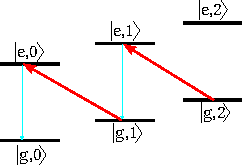
\includegraphics[width = 0.8\textwidth]{main/coolingScheme.pdf}
    \caption{Illustration of the concept behind sideband laser cooling. The laser (red) is detuned with respect to the electronic transition, by exactly $\omega_z$. Thus transitions are driven at the cost of a phonon. The atom is most likely to decay to the same Fock state, effectively causing it to lose phonons, as several excitations occur. This makes the ion "climb down the ladder" until it reaches the quantum ground state.}
    \label{fig:SBC}
\end{figure}

\section{Coupling of motional modes to enhance cooling}
\label{sec:Coupling}
As mentioned in both \cref{sec:Doppler} and \cref{sec:SBC}, laser cooling becomes very difficult once the charge-to-mass ratios of the two differ considerably. The reason for this is relatively easy to understand.
Since the laser cooling only interacts with the atomic ion, this is the only ion whose motion is cooled through the interaction with the light. In the case where the ions have similar charge-to-mass ratios however, their motions are so strongly coupled, that any cooling of the atomic ion, will cool the molecular ion as well.
As the ratios start to differ the motions quickly become uncoupled, and thus the cooling of the atom, no longer affects the molecule in any appreciative way. This is clearly seen on \cref{fig:WCMSCM}, which shows the temperature of Ba$^+$ ion, cotrapped with a polyporphyrine ($m_2 = 9000$ amu, $q_2 = 24$e). The blue curve shows the temperature of the motional modes, that have a large contribution from the atom. Clearly these modes are effectively cooled. In stark contrast we have the orange curve, which displays the temperature of all the modes that have low contribution from the atom, whose temperature remains effectively unchanged.

\begin{figure}
    \centering
    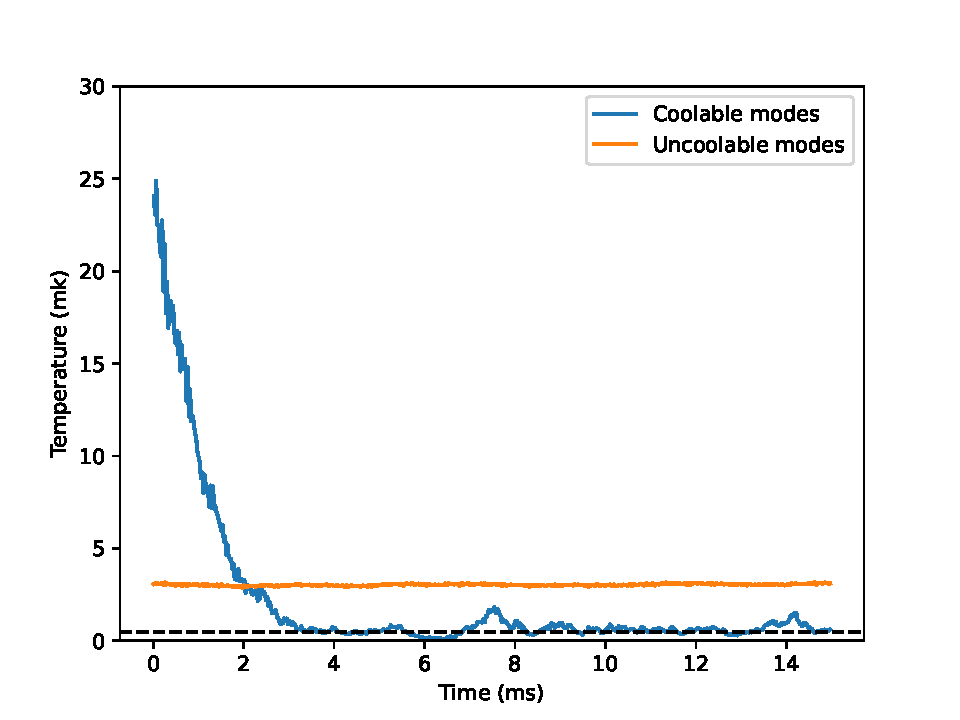
\includegraphics[width = \textwidth]{main/WCM_SCM_Temp.pdf}
    \caption{Simulation of Doppler cooling of a two/ion system, containing of a Ba$^+$ ion, and a polyporphyrin. Two curves are plotted, corresponding to the tempearture of the modes with high (blue), and low (orange) participation from the Ba$^+$ ion. Clearly only the modes with a high participation are cooled by the Doppler cooling}
    \label{fig:WCMSCM}
\end{figure}

In fact, this problem reaches further than simply cooling. For example, it is the molecular ion we wish to investigate with photon recoil spectroscopy (PRS). However the momentum kick gained from absorption on the molecule, will predominantly excite the motional modes with high participation from the molecule.
Unfortunately the readout method for PRS is very similar to the side-band pulses described in \cref{sec:SBC}, and thus for the same reasons, readout becomes impossible when the coupling grows too weak, since these modes have very small participation from the atomic ion, on which readout is performed.


The solution to this problem is to find some way to couple the two modes, allowing for the transfer energy from one to the other. Curiously enough the need for coupling such modes was present in Penning traps many years ago, in order to cool the so-called magnetron mode of such a trap \cite{PenningTrap,DehmeltPenningCool}. For the Pennin trap the solution found was to add another quadrupole field, oscillating at the frequency difference between the two modes to be coupled, such a solution also works for the case of the Paul trap as has been demonstrated very recently \textcolor{red}{CITE REFEREE}.

It is easiest to understand the coupling that occurs, when we consider the quantum mechanical case. Suppose we introduce some additional potential (by modulating a slight additional voltage on the endcap electrodes)
\begin{equation}
    V'(z_1,z_2,t) = \frac{\kappa V_0}{z_0^2}(q_1z_1^2+q_2z_2^2)\cos{\big([\omega_i-\omega_o]t\big)}\label{eq:couplingPot},
\end{equation}
where $V_0$ is the additional voltage put onto the endcap electrodes. We note that $V_0$ is kept small with respect to $V_{DC}$, such that the eigenmodes of the system are not considerably changed.

If we perform a Taylor expansion to second order around the equilibrium (at $V_0= 0$) positions is performed similarly to \cref{sec:2Ion}, we may write (neglecting the offest term)
\begin{align}
    V'(\delta z_1,\delta z_2,t)\approx &\frac{\partial V'}{\partial z_1}\bigg\vert_{eq}\delta z_1+\frac{\partial V'}{\partial z_2}\bigg\vert_{eq}\delta z_2
    +\frac{1}{2}\frac{\partial^2 V'}{\partial z_1^2}\bigg\vert_{eq}\delta z_1^2\nonumber\\+&\frac{1}{2}\frac{\partial^2 V'}{\partial z_2^2}\bigg\vert_{eq}\delta z_2^2
    +\frac{\partial^2 V'}{\partial z_1\partial z_2}\bigg\vert_{eq}\delta z_1\delta z_2.
\end{align}
For now, we only wish to consider the coupling of the modes, and thus neglect the first-order terms. Clearly these terms cannot couple the modes as $\delta\hat{z}_j\propto (\alpha_{j,o}\hat{a}_o+\alpha_{j,i}\hat{a}_i)+h.c.$ is not sufficient to transfer energy from one mode to another. If we instead consider solely the 2nd. order terms we find
\begin{align}
    \hat{V}'^{(2)} = \nonumber \frac{\hbar\kappa V_0}{2z_0^2}\cos{\big([\omega_i-\omega_o]t\big)}\bigg(&q_1\big(\frac{\alpha_{1,i}(\hat{a}_i+\hat{a}_i^\dagger)}{\sqrt{m_1\omega_i}}+\frac{\alpha_{1,o}(\hat{a}_o+\hat{a}_o^\dagger)}{\sqrt{m_1\omega_o}}\big)^2\\
    &+q_2\big(\frac{\alpha_{2,i}(\hat{a}_i+\hat{a}_i^\dagger)}{\sqrt{m_2\omega_i}}+\frac{\alpha_{2,o}(\hat{a}_o+\hat{a}_o^\dagger)}{\sqrt{m_2\omega_o}}\big)^2\bigg).
\end{align}
If the cosine is expanded using Euler's formula, and we move to the interaction picture, keeping only the non-rotating terms, we may massage the expression and eventually arrive at
\begin{equation}
    \hat{V}'^{(2)}_I = \frac{\hbar\kappa V_0\alpha_{1,o}\alpha_{1,i}}{4z_0^2\sqrt{\omega_i\omega_o}}\big(\frac{q_1}{m_1}-\frac{q_2}{m_2}\big)(\hat{a}_o^\dagger \hat{a}_i + h.c.),
\end{equation}
for which it is clear that the two modes of motion are coupled. We define $g_0 = \frac{\kappa V_0\alpha_{1,i}\alpha_{1,o}}{4z_0^2\sqrt{\omega_i\omega_o}}(\frac{q_1}{m_1}-\frac{q_2}{m_2})$, that we may write the coupling potential as 
\begin{equation}
    \hat{V}_I'^{(2)} = \hbar g_0(\hat{a}_i^\dagger \hat{a}_o + h.c.).
\end{equation}
It can be shown, that in the coupled system the time-dependent operators $\hat{a}_{i/o}^\dagger(t)$, are given by \cite{hou2022coherently}
\begin{align}
    &\hat{a_i}^\dagger(t) = \hat{a}_i^\dagger(0)\cos(g_0t) + i\hat{a}_o^\dagger\sin(g_0t),\\
    &\hat{a_o}^\dagger(t) = \hat{a}_o^\dagger(0)\cos(g_0t) + i\hat{a}_i^\dagger\sin(g_0t).
\end{align}
For which it is particularly interesting to note that for times $\tau_n = \frac{(2n+1)\pi}{2g_0}$, where $n$ is an integer, we find that $\hat{a}_i^\dagger(\tau_n) = \hat{a}_o^\dagger(0)$, and similarly for $\hat{a}_o^\dagger(\tau_n)$. In addition, we may write any arbitrary state of the system as
\begin{equation}
    \vert \Psi(t)\rangle = \sum_{m,n = 0}^\infty \frac{c_{mn}}{\sqrt{m!n!}}\big(a_i^\dagger(t)\big)^m\big(a_o^\dagger(t)\big)^n\vert 0\rangle_i\vert 0\rangle_o,
\end{equation}
where the time-dependance of the system is fully captured by the creation operators \cite{hou2022coherently}, the values $c_{mn}$ are determined by the initial state of the system, and $\sum c_{mn} =1$.
The action of the coupling is thus clear. In general the cause the two states to oscillate in and out of entanglement, and specifically for times $t = \tau_n$ the states for the two modes become swapped.
This is very beneficial for cooling, since we may cool the mode with high participation from the Ba$^+$ ion, perform a swap, and then cool again. This procedure should, in principle, lead to both modes being in their ground states.


The mode coupling also exists in the classical regime. \Cref{fig:polyPorCooling} shows a simulation of Doppler cooling of a system consisting of a  Ba$^+$ ion, and a polyporphyrin, while the coupling $V'$ is turned on. The results from this simulation stand in stark contrast to those of \cref{fig:WCMSCM}, where the temperature of the molecule is largely unchanged.
\begin{figure}[h]
    \centering
    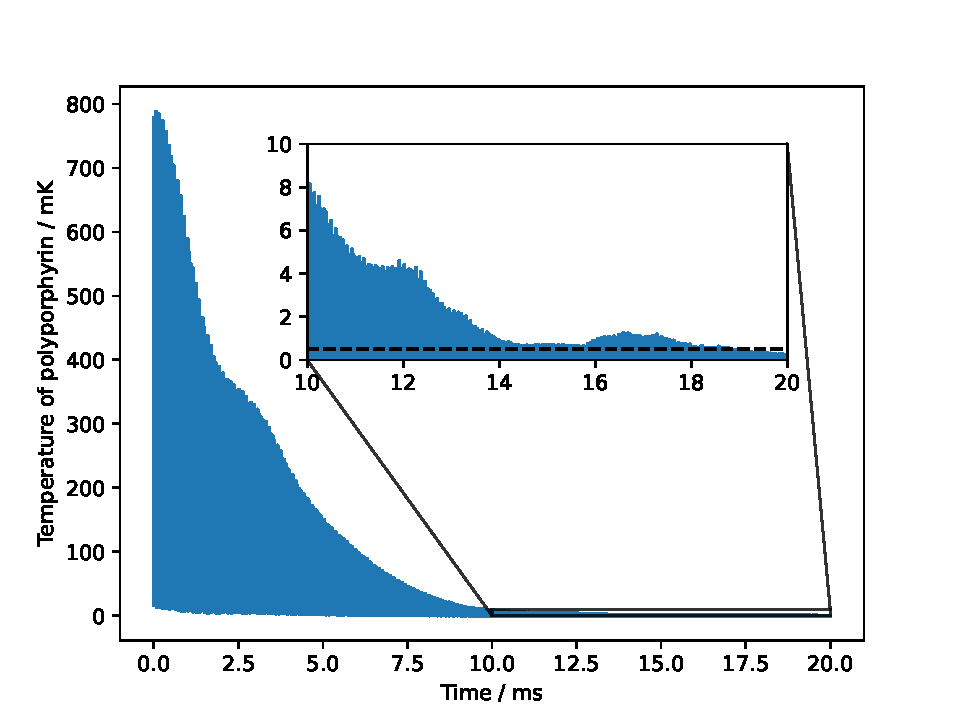
\includegraphics[width = 0.8\textwidth]{main/PolyPorCooling.pdf}
    \caption{Simulation results for Doppler cooling of a system consisting of Ba$^+$ ion and polyporphyrin, while the coupling potential from \cref{eq:couplingPot} is turned on. Unlike the case with no coupling \cref{fig:WCMSCM}, the molecule is cooled efficiently.
    The inset shows temperatures in the span $ t = $10ms to $t = $20ms, as temperatures grow so small that they are not clearly seen on the full figure. The black dotted line shows $T = 0.5$mK, which is the Doppler temperature, calculated by \cref{eq:DopplerTemp}.}
    \label{fig:polyPorCooling}
\end{figure}

In the derivations of this chapter we have ignored the 1st order terms of the Taylor expansion of the potential. In reality, these terms will play a role in the dynamics of the system, since they drive the ions at a frequency, which is similar to their motional frequencies. There are several ways to combat these first order driving terms.
One option, which has been implemented for the case of segmented microtraps, is engineering the field curvature in order to ensure the first order derivatives go to zero at the equilibrium locations of the ions \cite{WeaklyCoupled}. 

Since our trap has considerably fewer segments, such an approach is expected to be difficult to realize in our setup.
The second approach accepts that the driving terms will lead to heating, but attempts to move this heating into the modes, which are easily cooled, i.e. the ones with high participation from Ba$^+$. This can be done by biasing voltages slightly, such that the transfer potential $V'(z_1,,z_2,t)$ has its minimum at $z_{2,eq}$, instead of $z=0$.
We believe this would be relatively simple to implement in the current trap, as a similar thing is already done in order to compensate for micromotion.



The usefulness of this mode-coupling doesn't stop at laser cooling. As mentioned previously when performing PRS, we will largely excite the motion of the molecule, due to the absorption of light via the molecule. Mode-coupling allows for the efficient mapping of the motion of the molecule onto the motion of the ion, resulting in much higher measurement efficiency, and speed.


In addition to the contents of this report, the contents of \cref{chap:LinTrap} and the current chapter have also been used in the authoring of a paper, proposing an experiment to set bounds on a quantum collapse model, known as the continuous spontaneous localization model \cite{lenlereriksen2023testing}. Using the theory of \cref{sec:2Ion}, we found the strongest bounds on the models parameters could be set by performing measurements on the modes with high participation from the molecular ion, yielding another case where mode-coupling can be highly beneficial.




% Future work
%% ============================================================================
%%
%%  Part A / PhD Progress Report
%%
%%  Author: Jakob Lysgaard Rørsted (Mosumgaard)
%%
%%  Future work and outlook
%% ============================================================================

\chapter{Conclusion and outlook}
\label{chap:future}
In conclusion, we have derived the dynamics of systems consisting of one or two ions within a linear Paul trap, including their frequencies and motional modes. Importantly, we've found that if the charge-to-mass ratios of the ions differ significantly, their motions become largely uncoupled.

We've given an overview of the electrospray setup, which will be used for bringing molecular ions into the Paul trap. Additionally, we've performed several measurements on the first octopole, in order to characterize its behaviour.
In particular, we've found that loading fewer ions into the octopole results in cooler ions, and we've measured the life-time of ions stored in the octopole, finding that they may be stored there on the timescale of hours. This should allow us to fill the octopole with ions at the start of the day, and to keep using it as a secondary ion source, for experiments.

Finally, we've discussed both Doppler and sideband laser cooling of two-ion systems, and how cooling becomes unfeasible if the ions' motion becomes uncoupled. In order to solve this issue, we have proposed a scheme, which couples the two motional modes by introducing an additional weak quadrupolar potential, which oscillates at the frequency difference of the two modes.
We have presented an example simulation of Doppler cooling of a polyporphyrin cotrapped alongside Ba$^+$, which shows such a method will allow us to cool a molecular ion to the Doppler limit.


For sideband cooling, we have shown that such a coupling field will cause the states of the two modes to oscillate in and out of entanglement over time, and that at specific times, the coupling field will have the effect of a SWAP gate, swapping the states of the two modes. This will allow for sideband cooling of all modes.


There is of course still much work to be done.
Since January 2024, we have no longer been able to measure any ions at the last channeltron detector in the setup (see \cref{fig:esiDrawing}). We believe this is due to a mistake in the mounting of the push/pull feed-through of the first channeltron.  Mounted on the front of the first channeltron, there is a mesh with a circular hole below the detector, such that when the detector is pulled out of the ion beam, the ions will pass through the center of this hole, and experience symmetric surroundings, so as to avoid any deflection of the ion beam.
However, measurements show that the settings used for experiments would not have had the ions passing through the center of the hole in the mesh, but rather just past the edge. If even a small shift has happened it is possible that the ions are now simply hitting the mesh altogether, giving a reason for why the ions cannot reach the latter half of the experiment.

The plan is to open up the channeltron over the course of the summer, in order to fix this issue, and obtain ions at the end of the setup once more.

When we once again have ions all the way through, we are going to start mapping out how well ions are transferred from the first to the 2nd half of the setup, and try to determine optimal parameters for transferring a single ion to the end of the setup.
Once we can reliably deliver one, or a few ions at the end of the setup, we are going to mount the octopole ion guide (see \cref{fig:fullSetup}) onto the cryogenic chamber, containing the linear Paul trap. We are then going to test protocols for moving ions through the ion guide, by attempting to move a Ba$^+$ ion to the end of the ion guide, and bringing it back into the trap.

If all the above things work, all that is left is to connect all the parts of the setup, and attempt to perform recoil spectroscopy on a molecular ion, which has a similar mass-to-charge ratio to barium.
%
% Bibliography and such stuff
%
\clearpage

% Change the sorting of references to NAME-YEAR-TITLE (see preamble for details)
\begin{refcontext}[sorting=nyt]
  \raggedyright[4em] \printbibliography
  
  % If you really want to compress the bibliography, do this instead...
  % \raggedyright[4em] {\addtolength{\beforechapskip}{-6\baselineskip}\printbibliography}
\end{refcontext}


%
% Appendix
%
%\appendix
%\include{app/app}

\end{document}